\subsection{Opgave 52}

Grafen for en funktion f er vist på nedenstående figur.

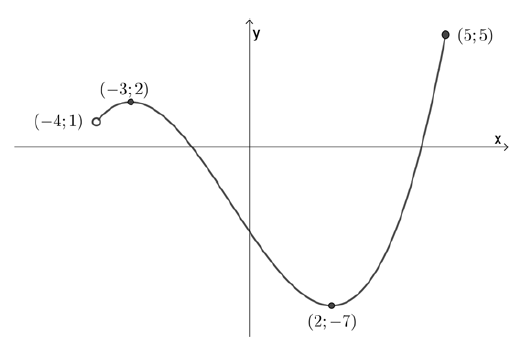
\includegraphics[width=8cm]{Opgave_51-56/Opgave_52/52.png}

Løs ligningen $f'(x) = 0$.

\ans

Når vi bliver bedt om at løse ligningen $f'(x) = 0$ bliver vi bedt om at finde de x værdier hvor hældningen på 
$f(x)$ er lig med 0. I de x værdier hvor hældningen for $f(x)$ er lig med 0 er de x værdier hvor tangenten i x værdien ville ligge horizontalt.
Dette sker typisk ved en funktions maksimums eller minimums punkter. I vores tilfælde kan vi se 2 x værdier hvor tangenten i de x værdier ville være horizontale.
Dette er tilfældet ved x værdierne $x = -3$ og $x = 2$. Det betyder at løsningen til ligningen $f'(x) = 0$ er 
$x = -3$ og $x = 2$. Tangenterne i de x værdier kan ses på figuren nedenfor  

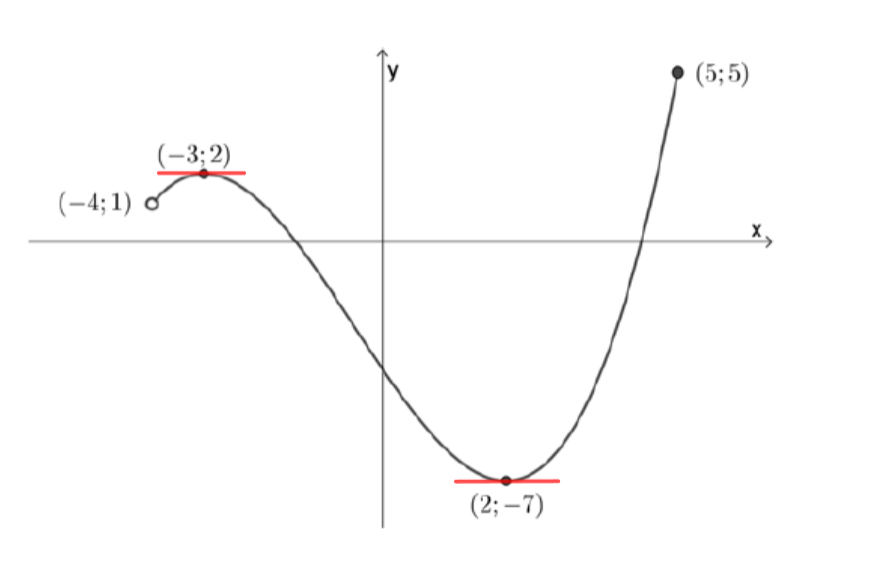
\includegraphics[width=8cm]{Opgave_51-56/Opgave_52/52.1.png}